\documentclass[letterpaper,12pt]{report}
\usepackage[top=1in,right=1in,bottom=1in,left=1.5in,includefoot,includehead]{geometry}

% PACKAGES
%**********
\usepackage{amsmath}		% AMS Math (http://www.ams.org/tex/amslatex.html)
\usepackage{amssymb}		% AMS Symbols
\usepackage{amsthm}			% AMS Theorems
\usepackage{tocloft}		% Format the Table of Contents
\usepackage{float}			% More float commands
\usepackage{sectsty}		% Format section and chapter headings
\usepackage{graphicx}		% Insert images in eps or pdf format
\usepackage{setspace}		% Line-spacing
\usepackage[bottom]{footmisc}	% Push footnotes to the bottom of the page

\usepackage{algorithmic}	% added by Jia to enable algorithms
\usepackage{algorithm}
\usepackage{natbib}
\usepackage{listings}

% Optional - link table of contents entries and citations
% LOAD THIS PACKAGE LAST!!! (Last of all usepackage commands)
% Feel free to change link colors
% \usepackage[linktoc=page,colorlinks=true,linkcolor=blue,citecolor=blue]{hyperref}


% OTHER USEFUL PACKAGES

% \usepackage{epsfig}		% For EPS figures
% \usepackage{subfigure}	% For side-by-side figures
% \usepackage{sidecap}		% Put captions on the side of figures
% \usepackage{rotating}		% Rotatiion of figures and tables
% \usepackage{multirow}		% Column and row spanning in tables
% \usepackage{chapterbib}	% Insert bibliograhpy with a simple include command
% \usepackage{color}		% Color text (see define below, in "Custom Definitions")
% \usepackage{enumerate}	% Special enumerated lists
% \usepackage[citestyle=numeric-comp,bibstyle=numeric,sorting=none]{biblatex}	% Newer citation system
% \usepackage[linktoc=page,colorlinks=true,linkcolor=blue,citecolor=blue,breaklinks]{hyperref}	% Hyper-linking of citations in the text and urls in the bibliography - IF YOU USE THIS PACKAGE, MAKE SURE IT IS BELOW ALL OTHER \usepackage{} ITEMS

% Generally, you will not want to edit this file, unless adding a LIST OF ILLUSTRATIONS (or similar)

\renewcommand\contentsname{TABLE OF CONTENTS}
\setlength{\cftbeforetoctitleskip}{0in}
\renewcommand{\cfttoctitlefont}{\hspace{\fill}\large\bfseries}
\renewcommand{\cftaftertoctitle}{\hspace{\fill}}

\renewcommand\listtablename{LIST OF TABLES} % Defines exact text of Title
\setlength{\cftbeforelottitleskip}{1in} % Defines how far down from the margin the title should be placed
\setlength{\cftafterlottitleskip}{0.25in} % Defines how far below the title the first entry will be
\renewcommand{\cftlottitlefont}{\hspace{\fill}\large\bfseries} % This line and the next define that the title should be centered and followed by a line with 'Table' on the left and 'Page' on the right.
\renewcommand{\cftafterlottitle}{\hspace{\fill} \vskip 10mm {\large Table \hspace{\fill} Page}}

\renewcommand\listfigurename{LIST OF FIGURES}
\setlength{\cftbeforeloftitleskip}{1in}
\setlength{\cftafterloftitleskip}{0.25in}
\renewcommand{\cftloftitlefont}{\hspace{\fill}\large\bfseries}
\renewcommand{\cftafterloftitle}{\hspace{\fill} \vskip 10mm {\large Figure \hspace{\fill} Page}}

\renewcommand\cftpartdotsep{\cftdotsep}
\renewcommand\cftchapdotsep{\cftdotsep}
\renewcommand\cftsecdotsep{\cftdotsep}
\renewcommand\cftsubsecdotsep{\cftdotsep}
\renewcommand\cftsubsubsecdotsep{\cftdotsep}
\renewcommand\cftparadotsep{\cftdotsep}
\renewcommand\cftsubparadotsep{\cftdotsep}
\renewcommand\cftfigdotsep{\cftdotsep}
\renewcommand\cfttabdotsep{\cftdotsep}

\setlength{\cftbeforepartskip}{12pt}
\setlength{\cftbeforechapskip}{12pt}
\setlength{\cftbeforesecskip}{12pt}
\setlength{\cftbeforesubsecskip}{12pt}
\setlength{\cftbeforesubsubsecskip}{12pt}
\setlength{\cftbeforeparaskip}{12pt}
\setlength{\cftbeforesubparaskip}{12pt}
	% Lots of special formatting to make the ToC adhere to MU requirements

% CUSTOM DEFINITIONS
%********************
% \def\clr#1{\textcolor{red}{#1}} % Color text red by typing: \clr{This is some text.}

% change margin text font size to footnote
\let\oldmarginpar\marginpar
\renewcommand\marginpar[1]{\-\oldmarginpar[\raggedleft\footnotesize #1]%
{\raggedright\footnotesize #1}}

\begin{document}

\doublespacing % Double line-spacing ( or specify something like \setspacing{1.8} )
\allsectionsfont{\singlespacing} % Only body text needs double spacing, titles can be single spaced

\setcounter{page}{1}    
\pagenumbering{roman}

\thispagestyle{empty}

\vspace*{\fill}
\centerline{\large{\bf CALCULATING BOUNDS ON INFORMATION LEAKAGE}} % The title on the Title Page must be in all caps.
\centerline{\large{\bf USING MODEL-CKECINGG TOOLS}}
\vskip 10mm
\centerline{\rule{150mm}{0.2mm}} % You can adjust the length of the horizontal line here.
\vskip 10mm
\centerline{A Thesis presented to} % Choose Thesis or Dissertation
\centerline{the Faculty of the Graduate School}
\centerline{at the University of Missouri}
\vskip 10mm
\centerline{\rule{150mm}{0.2mm}}
\vskip 10mm
\centerline{In Partial Fulfillment}
\centerline{of the Requirements for the Degree}
\centerline{Master of Science} % Change to your degree
\vskip 10mm
\centerline{\rule{150mm}{0.2mm}}
\vskip 10mm
\centerline{by}
\centerline{JIA CHEN} % Your name on the Title Page must be in all caps.
\centerline{Dr. Rohit Chadha, Thesis Supervisor} % Edit advisor and choose Thesis or Dissertation
\centerline{JUL 2014} % The month is required to be capitalized.  Use the month and year of your graduation, not the month and year you defend.
\vspace*{\fill}
	% Input the Title Page (no page number, but counts as roman numeral 'i')
%\newpage
\thispagestyle{empty}

\vspace*{\fill}
\centerline{\copyright\  Copyright by Your Name 2011}
\centerline{All Rights Reserved}
	% Input the Copyright Page. You have to pay additional fees to have your thesis/dissertation registered with the government, so this page is disabled by default.  Remove the % symbol before \input to re-enable it. For more information, see: http://gradschool.missouri.edu/policies/thesis-dissertation/guidelines/other-sections-ch6.php#copyright
\newpage
\thispagestyle{empty}

The undersigned, appointed by the Dean of the Graduate School, have 
examined the thesis entitled: % Choose thesis or dissertation

\vspace{6mm}
\centerline{CALCULATING INFORMATION LEAKAGE} % The title on the Title Page must be in all caps.
\centerline{USING MODEL CHECKING TOOLS}
\vspace{6mm}
\noindent presented by Jia Chen, % Edit with your name (does not need to be in all caps.)

\noindent a candidate for the degree of Master of Science % Change to your degree
and hereby certify that, in their opinion, it is worthy of acceptance.
\vskip 12mm
\centerline{\rule{100mm}{0.2mm}}
\centerline{Dr. Rohit Chadha} % Edit advisor
\vskip 10mm
\centerline{\rule{100mm}{0.2mm}}
\centerline{Dr. Prasad Calyam} % Edit committee member 1
\vskip 10mm
\centerline{\rule{100mm}{0.2mm}}
\centerline{Dr. Michela Becchi} % Edit committee member 1
% \vskip 10mm
% \centerline{\rule{100mm}{0.2mm}}
% \centerline{Dr. Committee Member} % Edit committee member 1
% \vskip 10mm
% \centerline{\rule{100mm}{0.2mm}}
% \centerline{Dr. Committee Member} % Edit committee member 1
	% Input the Approval Page (no page number)
\newpage
\pagenumbering{roman}
\setcounter{page}{2}
\addcontentsline{toc}{chapter}{ACKNOWLEDGMENTS} % This is the American english spelling (no E between G and M)

\centerline{\bf \large ACKNOWLEDGMENTS}
\vskip 10mm % Edit everything below with your acknowledging text.
This page is where you would acknowledge all those who helped you with your academic research. This is not necessarily where you would recognize loved ones who supported you during your studies. That would be more appropriately done in an optional Dedication page. I would like to thank Professor Smith � Lorem ipsum dolor sit amet, consectetuer adipiscing elit. Vestibulum eu tellus. Nullam et odio eget sapien porttitor interdum. Donec vel ante. Maecenas in sem a nunc viverra hendrerit. Quisque ut massa quis pede blandit pharetra. \par
Pellentesque sed ligula sit amet ligula scelerisque sagittis. Nulla adipiscing tellus at pede. Cras id nunc vel diam congue dictum. Donec a nulla nec eros ornare consequat. Nullam quis orci. Nam adipiscing, erat in congue pellentesque, dolor eros euismod quam, a egestas mauris magna varius justo. \par
Sed eu sem et lorem blandit volutpat. Duis pulvinar, arcu quis suscipit convallis, ante elit auctor dui, in fermentum diam velit a mauris. In risus odio, consectetuer quis, ullamcorper in, rutrum ut, metus.
	% Input the Acknowledgement Page (roman numeral page number 'ii')
% Only edit this file if you want to include a new list of illustrations, theorems, or other (in which case you will need to add a block to Command_Mods.tex

% Generate a table of contents
\newpage
\singlespacing
\tableofcontents
\doublespacing

% Generate a list of Tables and a list of Figures:
\newpage
\phantomsection
\addcontentsline{toc}{chapter}{LIST OF TABLES}
\listoftables

\newpage
\phantomsection
\addcontentsline{toc}{chapter}{LIST OF FIGURES}
\listoffigures
	% Generate and input a Table of Contents and List of Figures/Tables/etc.(roman numeral page number 'iii')

% !TEX root = ThesisMaster.tex
\newpage
\addcontentsline{toc}{chapter}{ABSTRACT}

\centerline{\bf \large ABSTRACT}
\vskip 10mm 

A confidential program should not allow any information about its secret inputs to be inferred from its public outputs. As such confidentiality is difficult to achieve in practice, it has been proposed in literature to evaluate security of programs by computing the amount of information it leaks. In this thesis, we consider the problem of computing information leaked by a deterministic program and use the information-theoretic measure of min-entropy to quantify the amount of information.

The main challenge in computing information leakage by a program using min-entropy is that one has to count the number of distinct outputs by that program. We find a polynomial-time reduction from the problem of counting outputs to the problem of checking safety in programs. Thus we propose a hypothesis that we can estimate leakage using model checking tools which are originally developed for checking safety.

We test the above hypothesis using two popular model checking tools, JMoped and Getafix. Our tests indicate that they do not scale as the number of bits in the input increases. However, we find that if the program enjoys the additional property of monotonicity then we can use a different reduction to the problem of checking safety. We observe a dramatic improvement in performance with this new reduction.

\iffalse

A \emph{confidential} program should not allow \emph{any} information about its secret inputs to be inferred from its public outputs.  As such confidentiality is difficult to achieve in practice, it has been proposed in literature to evaluate security of programs by computing the \emph{amount} of information leaked. %(a low amount of information leakage is desirable). 
We consider the problem of \emph{computing} 
information leaked by a deterministic  program  when the information-theoretic measure of \emph{min-entropy} is used to quantify the amount of information. 

The main challenge in computing the amount of  information leaked by a program $P$ using min-entropy is that one has to count the number of distinct possible outputs that may be observed when the program is run on different inputs. There is a polynomial-time reduction from the problem of checking whether information leaked by a program is equal to  (or less than) a given number to the problem of checking safety in  programs.  Thus, %in principle,   
it has been hypothesized that leakage can be estimated using model-checking tools which were  originally developed for checking safety in programs.  
 
We tested the above  hypothesis using two popular model-checking tools, JMoped and Getafix. Our tests indicate that these   do not scale as  the number of bits
in the input increases.  However, we show that if the program $P$ enjoys the additional property of \emph{monotonicity} then we can use a different reduction to the  problem of checking safety in  programs.  Note that if the program $P$ inputs $n$ bits and outputs $m$ bits then the program $P$ can be considered as  a function $P_{func}$ from $n$-bit binary numbers to $m$-bit binary numbers.    We say $P$ enjoys   
\emph{monotonicity}  if $P_{func}$ is monotonic. %ally increasing.
%if for each pair of $n$-bit  binary numbers $s_1, s_2$  such that  $s_1\leq s_2,$ we have that %$P_{func}(s_1) \leq P_{func}(s_2).$ 
We observe a dramatic improvement in the performance with this new reduction.

\fi

  

\newpage
\setcounter{page}{1}
\pagenumbering{arabic}
\addtocontents{toc}{\bigskip \textbf{CHAPTER}\par}

% !TEX root = ThesisMaster.tex


\chapter{Introduction}
	\label{CH_Intro}

A desirable property for a program is \emph{non-interference}~\cite{GougenMeseguer,Reynolds} which informally says that a program should  never leak  any information about its secret inputs. Formally, \emph{non-interference}~\cite{GougenMeseguer,Reynolds}
 says that the \emph{low-security observations} of the executions of a program must be independent of secret inputs. However, the desired functionality of a program usually makes non-interference unachievable. For example, a password checker behaves differently on a correct password and an incorrect password   (and its behavior even depends on the number of incorrect passwords
entered).   Therefore,  many authors~\cite{Denning,Gray,Millen,Smith} have proposed to evaluate security of programs by  quantifying the amount of information leaked. How do we measure the amount of information leaked? How to compute the information leaked?


For measuring the amount of information leaked by programs, information-theoretic measures are often used. In this approach, a program is modeled as an information channel that  {transforms} a random variable taking values from the set of confidential inputs into a random variable taking values from the set of public outputs.  Then information-theoretic measures are used to quantify the adversary's initial certainty about the secret inputs and  the  uncertainty remaining in the secret inputs after the adversary observes  the execution.
 The amount of information leaked by the program is the difference between the two. While, many information-theoretic measures can be used, it has been argued that leakage based on min-entropy is appropriate to security applications~\cite{Smith}.   Intuitively, leakage based on min-entropy measures vulnerability of the secret inputs to a \emph{single} guess of the adversary who observes the program execution.
 

Even though quantifying information leaked in programs is appealing, it is however not easy to compute information leaked in programs. Indeed it is known that the decision problem of checking whether information leaked  in non-recursive boolean programs is equal to (or less than) a given rational number is  {\PSpace}-complete~\cite{Jp2,Jp3,POST,Krish}. Recall that 
 {\PSpace} is the class of decision problems that can be solved by Turing machines that accesses at most a  polynomial number of cells on its working tape and that this class includes {\textsf{NP}} decision problems. 
 
 
 

In order to measure the information leaked by a program $P$ using min-entropy, one has to count the number of different possible outputs that may be achieved when the program is run with different inputs. The amount of information leaked is the binary logarithm of this number, 
Now, if the  input to the program $P$ consists of $n$-bits, this quantity can be computed by running the program on each of the  $2^n$ different inputs and remembering the outputs observed on each of the different inputs.  Since different inputs can lead to different outputs, this naive algorithm can take $2^n$-additional space.
This naive algorithm (which we shall call algorithm A for the rest of the section) has exponential time and exponential space complexity.  The same computation can be actually carried out in polynomial additional space by using nested iteration.
The outer iteration ranges over  all possible outputs and checks if there is an input that leads to that particular output by iterating over all possible inputs. Hence, in this alternative algorithm, the program has to be run $2^{2n}$ times.  The latter observation  immediately leads to the result that  the decision problem of checking whether information leaked  in non-recursive boolean programs is  equal to (or less than) a given rational number in {\PSpace}. Indeed, the latter algorithm (which we shall call algorithm B for the rest of the section)  provides an immediate polynomial-time reduction to the problem of checking whether the program counter reaches a given location in a program, which is also known to be {\PSpace}-complete.  


Now,  algorithm A for computing min-entropy takes above takes  at least exponential time and exponential space, while  algorithm B takes at least exponential time. Hence, they do not scale
very well  as $n$, the number of input bits increase.  However, it has been suggested in 
~\cite{POST} that one can potentially exploit the polynomial-time reduction to the reachability problem in order to estimate the amount of information leaked by using modelchecking tools as modelchecking tools were originally developed for checking whether a particular state in a program is reachable (on any possible input). These modelchecking tools do not explicitly run the program on all inputs. Instead use a variety of heuristics to solve the reachability problem. 


We tested the above  hypothesis using two popular model-checking tools, jMoped~\cite{Jmoped} and Getafix~\cite{getafix}. 
Jmoped is a tool developed for checking reachability in Java programs. The key technology used in JMoped is the use of Binary Decision Diagrams (BDDs)~\cite{lee,Bry86}. BDDs are data structures designed to efficiently   store Boolean functions. In jMoped, the input program is translated  as set of \emph{transitions} on the states of the program (a state of a non-recursive program is the current line number and the values of the variables of the program). Each transition  then models how program execution changes the state of the program.  However, instead of writing transitions explicitly,
BDDs are used to store the set of transitions.  Reachability can then be encoded as  the least fix-point solution of a set of Boolean equations which can be solved with efficient BDD operations. Getafix~\cite{getafix} is based on similar ideas except that it accepts only Boolean programs and reachability is encoded as a winning condition on a 2-player game on a  transition system. Although, these tools should work in theory, our tests for estimating min-entropy indicate that these do not scale very well  as the number of bits in the input increase. 


However, we  identified a condition under which there is a dramatic improvement in the performance of these tools. In particular, we show that if the program $P$ whose information leakage we are estimating satisfies the additional property of \emph{semi-monotonicty} then the computation of min-entropy becomes more feasible. Note that  
  if the program $P$ inputs $n$ bits and outputs $m$ bits then the program $P$ can be considered as  a function $P_{func}$ from $n$-bit binary numbers to $m$-bit binary numbers. Recall that the function $P_{func}$ is monotonically increasing  if  for each pair of $n$-bit  binary numbers $s_1, s_2$  such that  $s_1\leq s_2,$ we have that $P_{func}(s_1) \leq P_{func}(s_2).$ Note that a monotonically increasing  function we have that for each $n$-bit binary number $s$, $P_{func}(s) \geq \max_{ s'\leq s} {P_{func}(s')}.$
    We say the the program $P$ is semi-monotonically increasing if for each $n$-bit  binary number $s$ either $P_{func}(s) \geq \max_{ s'\leq s}{P_{func}(s')}$ or $P_{func}(s) \in \set{P_{func}(s') \mathbin{|} s'\leq s}.$ We can similarly define semi-monotonically decreasing programs. The program $P$ is said to be semi-monotonic if $P$ is either 
    semi-monotonically increasing or decreasing. 

The key observation that we exploit is that for semi-monotonicty we can essentially use algorithm A for computing information leakage except that we do not need to use exponential additional space. Instead, if the program $P$ is semi-monotoncially increasing (increasing respectively) then while iterating over the inputs,  we just need to remember in each iterative step  the total number of the distinct outputs seen thus far as well as the highest  (lowest respectively) output seen thus far. Thus, for semi-monotonic programs we have a new polynomial-time reduction of the decision problem of checking whether information leaked  in non-recursive boolean programs is  equal to (or less than) a given rational number to the problem of checking whether a line number in a program is reachable or not.  We now use this new reduction to estimate the information leaked in programs using jMoped and Getafix and  observe a dramatic improvement in their performance with this new reduction.



  
 
%
\paragraph{Related work.}
\label{sec:related}
The \emph{complexity} of computing the amount of leakage in Boolean programs has been   considered recently in~\cite{Jp1,Jp2,Jp3,Krish,rch:mu:fsttcs2012,Krish,POST}. 
In recent years, several automated approaches from model checking \cite{BackesKopf,Kopf,Kostas07,Kostas08}, static analysis \cite{clark94,clark05,clark07,BackesKopf}, and statistical analysis \cite{Kopf,Chothia}  have been employed to compute information leakage. We mention the most closely related work.


~\cite{Plas11, Plas13} estimates min-entropy leakage using SMT solvers. SMT solvers are tools developed to check whether a given first-order formula over a decidable first-order theory has a solution or not.  In ~\cite{Plas11, Plas13}, the authors estimate an upper bound of number of feasible outputs of a program by iterating over each pair of output bits and computing how many different values of these output bits can be achieved (i.e., how many of the values $\set{00,01,11,10}$ can be actually observed).  This technique only yields an upper bound, and it is easy to construct examples where the upper bound is a very poor estimate of the actual value.
 


Another line of closely related work is the work on computing information leakage measure using Shannon entropy~\cite{BackesKopf,Malacria07}. In this line of work, 
Shannon entropy (and not min-entropy) is used to measure uncertainty of the adversary. Usually an assumption of uniformly distributed inputs is made. When Shannon entropy is used to measure information leakage, one has to compute not only the number of feasible outputs but one also has to compute, for each feasible output,  the number of inputs that lead to that particular output. In order to compute these two things, usually an  equivalence relation on inputs is defined as follows: two inputs are equivalent if they lead to the same output. Then one needs to compute these equivalence classes. In~\cite{BackesKopf}, these equivalence classes are constructed iteratively by first starting with a single equivalence class and progressively refining them until they can be refined no further. At each iteration,   the equivalence relation is characterized using logical formulas and the refinement step uses experimental runs. In \cite{Kopf}, statistical analysis is used for this construction. In ~\cite{Malacria07}, bounded model-checking is used to compute the equivalence. In bounded model-checking, reachability is checked assuming that the program executes at most a bounded number of steps. Hence, this method gives an approximate value of information leakage. 

%While we have chosen min-entropy as the measure of information, we note that the maximum amount of information leaked by deterministic programs under all possible apriori distributions on inputs, when   matches exactly the min-capacity. 
%
%
%
%
%Introduce the reader to the current problem that you wish to solve, and why anyone should care about it.
% !TEX root =  ThesisMaster.tex


\chapter{Theoretical background}
	\label{CH_02}

\section{Min-entropy and information leakage in programs}
% !TEX root =  ThesisMaster.tex

\newcommand{\calC} {\mathcal{C}}


We briefly recall the mathematical theory behind computation of information leakage in programs. 
For computing information leakage, a program is usually considered as an information-theoretic channel between its inputs and outputs. Formally, 
\begin{mydef}
An information-theoretic channel $\calC$ is a triple $(S,O, C_{SO})$ such that 
\begin{itemize}
\item  $S$ is a finite set of secret input values,
\item $O$ is a finite set of secret output values, and 
\item $C_{SO}$ is a $|S| \times |O|$ non-negative matrix such that $\sum_{o_\in O} C_{SO}(s,o) =1. $
\end{itemize}
$\calC$ is said to be deterministic if for each $s\in S$ there is a unique $o \in O$  such that $C_{SO}(s,o)=1.$
\end{mydef}

For $s\in S$ and $o\in O,$ the quantity $C_{SO}(s,o)$ is  the conditional probability of obtaining output
$o$  given that the input to the channel is $s$. 
Given any information-theoretic channel $\calC=(S,O, C_{SO})$ and \emph{apriori} distribution $Prob_S$ on $S$,   we get a joint probability distribution $Prob_{S,O}$ on 
$S\times O$ given as  
$ Prob_{S,O} ((s,o))= Prob_S (s) C_{SO} (s,o).$  For the purpose of this thesis, we shall associate with each deterministic program $P$, a  deterministic  channel $P_\calC= (S,O, C_{SO})$ 
where $S$ is the set of all possible secret inputs of $P$, $O$ is the set of all possible outputs of $P$ and  $C_{SO}(s,o)=1$ iff
the program $P$ outputs $o$ on input $s.$ 

When measuring information leakage in programs using min-entropy~\cite{Smith},  an adversary  is considered which tries to guess the input to the program before and after the program is executed.  The difference in \emph{uncertainty} about  $S$ before and after the program execution is taken to be the amount of information leaked. It was proposed in~\cite{Smith}
that min-entropy be used as the measure of uncertainty. We refer the reader to~\cite{Smith} for details regarding theoretical foundations behind min-entropy.  We just point out here the relevant formulas. 

\begin{mydef}
Let $\calC=(S,O, C_{SO})$ be an information-theoretic channel and let  $Prob_S$ be an apriori distribution on $S.$
 The initial uncertainty of the adversary, written  $ H_{\infty}(S) $, is taken to be $-\log_2 \max_{s\in S} Prob_S(s) $ and final uncertainty, written  $ H_{\infty}(S | O) $,  is taken to be $-\log_2 \sum_{o\in O} \max_{s\in S} Prob_{S,O}((s,o)).$ The amount of information leaked by $\calC$, written $L_{S,O}$ is
 $$ L_{S,O} =  H_{\infty}(S) - H_{\infty}(S | O).$$
\end{mydef}

As expected, the amount of information leaked by a program is said to be the amount of information leaked by the channel $P_\calC$ associated to it.  
We are interested in computing the maximum possible amount of leakage under all possible apriori distributions (this quantity is  also known as \emph{min-capacity}). It turns out that for deterministic programs, this just amounts to computing the number  of outputs that are actually feasible, i.e., are actually realized by some input.

\begin{mythm} (\cite{Smith}) Let $\calC=(S,O, C_{SO})$ be a deterministic channel. Let 
$feasible=\set{o\in O \mathbin{|} \exists s\in S.\ C_{SO}(s,o)=1}.$  Then for any apriori distribution $Prob_S$ on $S$, we have that the information leaked
$ L_{S,O} \leq \log_2 |feasible|.$ Furthermore $ L_{S,O} = \log_2 |feasible|$ if $Prob_S$ is the uniform distribution on $S.$
\end{mythm}

\begin{remark}
Sometimes, Shannon entropy is used to measure uncertainty instead of min-entropy. However, it was shown in~\cite{Smith}, that if we measure information leaked using Shannon entropy then Shannon capacity, the maximum amount of information leaked, of deterministic programs under all possible apriori distributions  matches exactly the min-capacity. 
\end{remark}

\section{The problem and two intuitive solutions}
We define a program $P$ as follows:
\begin{mydef}
Let $bitLength\in \left\{ {0,1,2,..., 32}\right\}$ and let $P$ be a function whose input $S \in \left\{ {0,1,2,..., 1\ll bitLength-1}\right\}$ and output $O \in \left\{ {0,1,2,..., 1\ll bitLength-1}\right\}$.
\end{mydef}

And we need to count the number of outputs of $P$. We come up with two approaches: 

\begin{enumerate}
\item Put the program in a double loop and count the number of outputs. The outer loop is for possible outputs and the inner loop is for inputs. When the program in the inner loop produces an output which matches the outer loop, counter increases.
\item Let the program iterate through all input values and record the output hit results in a bit array. Counter increases when a bit flips.
\end{enumerate}

The first approach is time-consuming, while the second one is memory-consuming. We will discuss these two approaches in detail in the subsections.

\subsection{Double loop}
In Algorithm \ref{alg:doubleLoop}, for each possible output value, we iterate through the input range to see if an input can result in this output. If we hit this output, $OCounter$ increases and the code breaks out of the inner loop to continue testing the next possible output value. After the double loop finishes, the value of $OCounter$ is the number of outputs of program $P$.

\begin{algorithm}
\begin{algorithmic}
\STATE $S \leftarrow 0$
\STATE $O \leftarrow 0$
\STATE $SIn \leftarrow 0$
\STATE $OOut \leftarrow 0$
\STATE $OCounter \leftarrow 0$

\STATE $SMax \leftarrow 1 << bitLength - 1$
\STATE $OMax \leftarrow 1 << bitLength - 1$

\FOR{$O=0$ to $OMax$}
\FOR{$S=0$ to $SMax$}
\STATE $SIn \leftarrow S$ 
\STATE $OOut \leftarrow P(SIn)$ 
\COMMENT{the program $P$ takes $SIn$ as input}
\IF{$OOut = O$}
\STATE $OCounter \leftarrow OCounter + 1$
\STATE break
\ENDIF
\ENDFOR
\ENDFOR
\end{algorithmic}

\caption[Double loop]{Calculate the number of outputs using double loop.}
\label{alg:doubleLoop}
\end{algorithm}

In this approach, we declare seven variables, and all of them require $bitLength$ bits except for $OCounter$ which needs to be $bitLength + 1$ bits. The total memory usage for variables is $7 \times bitLength + 1$ at $O(bitLength)$. As with execution time, we assume program $P$ takes $t(P)$ seconds to execute, and the total execution time for the double loop when break is never reached is $2^{bitLength} \times 2^{bitLength} \times t(P)$. Thus the time complexity is $(2^{O(bitLength)}) \times t(P)$.

In order to get an estimation of how much time the double loop will take to execute, we implemented a piece of C code with an empty while loop which loops $2^{32}$ times. On our experiment PC, this loop takes on average $10.30$ seconds to complete. Were we to run a double loop in bit length of 32, the execution time would be $2^{32} \times 10.30$ seconds, which is around $1403$ years. Running the double loop at 32 bits would be infeasible.

Starting with bit length $n$, the time requirement for a full double loop is $2^{2 \times n} \times t(P)$. Increase the bit length by one and the time becomes $4 \times 2^{2 \times n} \times t(P)$, four times the previous time. Table \ref{tab:gccRun} shows the actual execution time of an empty double loop under different bit length, and the time increase follows the theoretical analysis. At bit length of 23, the execution time would exceed a day, and executing at higher bit length is impractical.

\begin{table}
\centering
\begin{tabular}{|l|l|l|}
\hline Bit length & Time(s) & Multiplier\\
\hline 14 & 0.708 & 	\\
\hline 15 & 2.797 & 3.951	\\
\hline 16 & 11.196	& 4.003	\\
\hline 17 & 44.515	& 3.976	\\
\hline 18 & 178.970	& 4.020	\\
\hline 
\end{tabular}
\caption{Execution time of an empty double loop with different bit length.}
\label{tab:gccRun}
\end{table}

\subsection{Single loop and array}
In Algorithm \ref{alg:singleLoop}, we create a bit array with size equal to the maximum number of possible outputs($1 << bitLength$, or $2^{bitLength}$) and initialize it with zeros. While we iterate through the range of $S$, we set each $OHit[P(SIn)]$ to $1$. When a $0$ turns to $1$, we increase $OCounter$. After the loop, the value of $OCounter$ is the number of outputs by program $P$. 

\renewcommand{\algorithmiccomment}[1]{// #1}
\begin{algorithm}
\begin{algorithmic}

\STATE $S \leftarrow 0$
\STATE $O \leftarrow 0$
\STATE $SIn \leftarrow 0$
\STATE $OOut \leftarrow 0$
\STATE $OCounter \leftarrow 0$

\STATE $SMax \leftarrow 1 << bitLength - 1$
\STATE $OMax \leftarrow 1 << bitLength - 1$
\STATE $OHit[OMax + 1] \leftarrow [0]$

\FOR{$S=0$ to $SMax$}
\STATE $SIn \leftarrow S$ 
\STATE $OOut \leftarrow P(SIn)$ 
\COMMENT{the program $P$ takes $SIn$ as input}
\IF{$OHit[OOut] = 0$}
\STATE $OCounter \leftarrow OCounter + 1$
\STATE $OHit[OOut] \leftarrow 1$
\ENDIF
\ENDFOR

\end{algorithmic}

\caption[Single loop]{Calculate the number of outputs using single loop and a table.}
\label{alg:singleLoop}
\end{algorithm}

In Algorithm \ref{alg:singleLoop} except for the array we have 7 variables using $7 \times bitLength + 1$ bits memory. The array $OHit[]$ is of size $2^{bitLength} \times 1$ bits making a total of $2^{bitLength} + 7 \times bitLength + 1$ bits at $2^{O(bitLength})$. As with execution time, we assume program $P$ takes $t(P)$ seconds to execute, and the execution time for the single loop is $2^{bitLength} \times t(P)$. Thus the time complexity is $(2^{O(bitLength)}) \times t(P)$.

We set the bit length to $32$. In array $OHit[]$, each element is $1$ bit and the number of elements is $2^{32}$. The total memory usage for this array is $2^{32} \times 1$ bits, which is $0.5$ gigabytes. To our knowledge, it is neither difficult nor expensive to build a PC with more than 16 gigabytes of memory, and we can get such a PC off-the-shelf from top gaming PC brands like Alienware. However, as this memory requirement grows exponentially, adding five or six bits to the bit length and the requirement will exceed the capacity of current PCs.

\subsection{Comparison}
Table \ref{tbl:execTime} and \ref{tbl:memReq} show a comparison on execution time and memory usage respectively for these two approaches. The single loop and array approach has exponential growth for both time and memory, while the double loop approach has exponential growth for time but linear growth for memory, so we choose the double loop approach. 

\begin{table}
\centering
\begin{tabular}{|l|l|l|}
\hline
 & Execution time & Growth  \\ \hline
Double loop & $2^{2 \times bitLength} \times t(P)$ & $\times 4$  \\ \hline
Single loop \& array & $2^{bitLength} \times t(P)$ & $\times 2$		\\ \hline
\end{tabular}
\caption{Comparison of the two approaches on execution time and their growth. $t(P)$ is the execution time of the program within the loop.}
\label{tbl:execTime}
\end{table}


\begin{table}
\centering
\begin{tabular}{|l|l|l|}
\hline
 & Memory requirement(bits) & Growth \\ \hline
Double loop & $7 \times bitLength + 1$ & +7 \\ \hline
Single loop \& array & $2^{bitLength} + 7 \times bitLength + 1$ & $+ 2^{bitLength} + 7$ \\ \hline
\end{tabular}
\caption{Comparison of the two approaches on memory requirement and their growth.}
\label{tbl:memReq}
\end{table}

\chapter{Experiment with Getafix}
	\label{CH_03}

\marginpar{(why and what other property are there)}
We want to use model-checking tools to see if we can reduce the time requirement of algorithm \ref{code:doubleLoop}. Specifically, we choose the reachability property and append algorithm \ref{code:reachLine} to the end of algorithm \ref{code:doubleLoop}. The statement within the if statement has a label. Although the exact statement following that label is irrelevant, reaching this line means $OCounter$ satisfies the constrains in the condition block.

\marginpar{correct citations of web page}
We experimented on several model-checking tools, including Interproc from \cite{_interproc_2011}, Berkeley Lazy Abstraction Software Verification Tool(Blast) from \cite{_mtc_2008} and Getafix from \cite{la_torre_analyzing_2009}. We can not get correct reachability results from Interproc and Blast, so we shift our focus on Getafix.

\renewcommand{\algorithmiccomment}[1]{// #1}
\begin{algorithm}
\begin{algorithmic}

\IF{value of $OCounter$ meets certain constrains}
\STATE reach: $OCounter$
\COMMENT{a label followed by a statement}
\ENDIF

\end{algorithmic}

\caption[Single loop]{Determine if $OCounter$ meets certain constrains.}
\label{code:reachLine}
\end{algorithm}

\section{Getafix}
Getafix is a symbolic model checker for Boolean programs implemented in \cite{la_torre_analyzing_2009}. Getafix only supports reachability check. It translates sequential and concurrent Boolean programs into Boolean formulae and uses the model-checker Mucke to solve the reachability problem symbolically using Boolean Decision Diagrams \cite{_getafix_2009}. 
\marginpar{Mostly copied from getafix website. Need rewrite}

\section{The converter}
Input for Getafix are boolean programs, meaning it only supports binary variables which can be either 0 or 1. We represent our problem in c-style code, thus we need to translate it into boolean form. We implemented a converter to automate this process. The converter has three components, a parser, a built-in function generator and a piece of script which calls the first two components and assemble the output file.

Input to the parser is the c-style code file and the desired bit length. Output of the parser is its corresponding boolean program which follows the syntax of Getafix input file. First we define the syntax of input code to the parser and second we create the parser using flex and bison. The parser scans the input code and builds a syntax tree. Then the parser prints the syntax tree as a boolean program. The parser has three points worth noting:

\begin{enumerate}
\item When printing the output code, the parser ``stretches'' each variable and literal into its binary form. Assume the desired bit length is $bitLength$. We split each variable into $bitLength$ variables by copying the name of the variable $bitLength$ times and append a counter value to each one. Also we convert a literal to its corresponding binary value and prepend it with zeros to reach the desired length.
\item In a boolean program, all operators operate on bit level, so we need to implement higher-level operators like plus, minus, greater than and left shift using operators that Getafix supports. In the parser, we print these high-level operators as function calls in the output boolean program, and the built-in function generator generates the body of the function.
\item In the boolean code syntax which Getafix defines, function call plus the semicolon is defined as a statement, and another rule allows the code to assign a function call to an identifier, but function call itself is not an expression. This means that a function call can not work as an expression as in many other languages, and it leads to two problems: First, the decider expression in if...else and while statements can not contain function calls. Second, parameters of a function call or operands to an operator can not be a function call. We automated a solution in the parser to the first problem, which assigns the decider expression to a temporary variable and use that variable as the decider, so we can use the c-style if...else and while in the input code. For the second problem, a possible solution would be to manage a set of internal temporary variables and assign each function call to a variable, but we did not implement it.
\end{enumerate}

\section{Tests and results}
\subsection{Sanity check}


\chapter{Experiment with Getafix and jMoped}
	\label{CH_04}

We want to use model-checking tools to see if we can reduce the time requirement of Algorithm \ref{alg:doubleLoop}. Specifically, we choose the reachability property and append Algorithm \ref{alg:reachLine} to the end of Algorithm \ref{alg:doubleLoop}. The statement within the if statement has a label. Although the exact statement following that label is irrelevant, reaching this line means $OCounter$ satisfies the constrains in the condition block.

We experiment on several model-checking tools, including Interproc from \cite{_interproc_2011}, Berkeley Lazy Abstraction Software Verification Tool (Blast) from \cite{_mtc_2008}, Getafix from \cite{getafix} and jMoped from \cite{moped}. We can not get correct reachability results from Interproc and Blast, so we shift our focus onto Getafix and jMoped.

\renewcommand{\algorithmiccomment}[1]{// #1}
\begin{algorithm}
\begin{algorithmic}

\IF{value of $OCounter$ meets certain constrains}
\STATE reach: $OCounter$
\COMMENT{a label followed by a statement}
\ENDIF

\end{algorithmic}

\caption[Single loop]{Determine if $OCounter$ meets certain constrains.}
\label{alg:reachLine}
\end{algorithm}

\section{Getafix}
Getafix is a symbolic model checker for Boolean programs. Getafix only supports reachability check. It translates sequential and concurrent Boolean programs into Boolean formulae and uses the model-checker Mucke to solve the reachability problem symbolically using Boolean Decision Diagrams. 

\begin{figure}
\centering
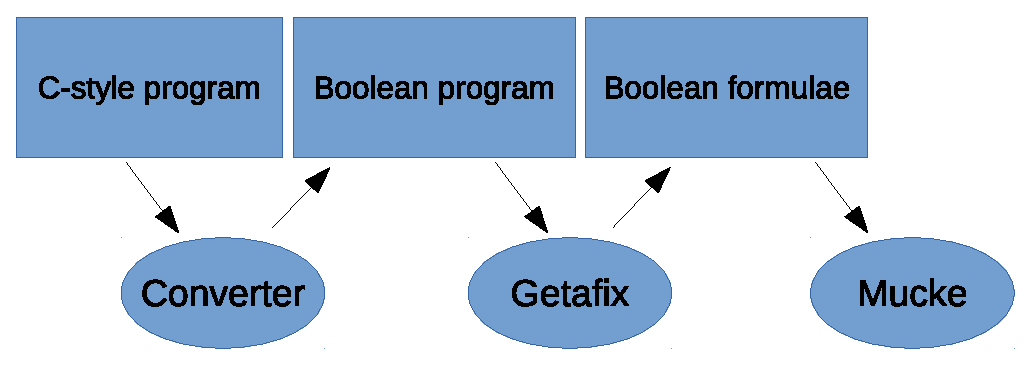
\includegraphics[scale=0.8]{Figures/workFlow}
\caption{Workflow of calculating information leakage with Getafix.}
\label{fig:workFlow}
\end{figure}

\subsection{The converter}
Input for Getafix are boolean programs, meaning it only supports binary variables which can be either 0 or 1. We represent our problem in C-style code, thus we need to translate it into boolean form. We implemented a converter to automate this process, and Figure \ref{fig:workFlow} shows the workflow we used to calculate information leakage using Getafix. The converter has three components, a parser, a built-in function generator and a piece of script which calls the first two components and assembles the output file. The converter has these properties:

\begin{enumerate}
\item The input to the converter is a C-style code file and a positive integer which represents the bit length. The converter supports 32 bits and less. Also note that the converter represents a number with bit length of $bitLength$ using $bitLength + 1$ bits. We do this so that we do not need to deal with the upper bound explicitly when writing a loop iterating from $0$ to $1<<bitLength - 1$.
\item The output of the converter is a boolean program which follows the syntax of Getafix input file.
\item In the language that we defined for the input file, we support only one variable type: non-negative decimal integer. Again we support the length up to 32 bits.
\item Our converter does not support function definitions. The input file has two parts, variable declarations block and statements block. The parser will print these blocks into the main function of the output boolean program. Also we require all variable declarations to appear before statements in the input code. Getafix input syntax has this requirement, and we decide to keep it in our converter.
\item We implement support for the following symbolic operators in the language: plus +, minus -, and \&, or $|$, xor \textasciicircum , greater than \textgreater, equal ==, less than \textless, not equal !=, greater than or equal \textgreater=, less than or equal \textless=, left shift \textless\textless and right shift \textgreater\textgreater.
\item We implement support for three control statements: if...else, while loop, goto and statements with labels. We currently do not support for loop, do...while loop, switch statements, break and continue, but these statements can be easily expressed using the supported ones.
\end{enumerate}

Input to the parser is a C-style code file and a desired bit length. Output of the parser is its corresponding boolean program which follows the syntax of Getafix input file. First we define the syntax of the input code and second we create the parser using flex and bison. The parser scans the input code and builds a syntax tree. Then the parser prints the syntax tree as a boolean program. The parser has three points worth noting:

\begin{table}
\caption{Examples of input and output of the parser, with bit length of 4}
\label{tbl:parser-example}
\begin{tabular}{|l|l|}
\hline
Input& Output  \\ \hline
var SMax = 16;     & \begin{tabular}[c]{@{}l@{}}decl SMax4,SMax3,SMax2,SMax1,SMax0;\\ Smax4, SMax3, SMax2, SMax1, SMax1 := 1,0,0,0,0;\end{tabular} \\ \hline
STemp = STemp - 5; & \begin{tabular}[c]{@{}l@{}}STemp4,STemp3,STemp2,STemp1,STemp0 := \\ minus(STemp4,STemp3,STemp2,STemp1,STemp0,0,0,1,0,1); \end{tabular} \\ \hline
\end{tabular}
\end{table}

\begin{enumerate}
\item When printing the output code, the parser ``stretches'' each variable and literal into its binary form. Assume the desired bit length is $bitLength$. We split each variable into $bitLength$ variables by copying the name of the variable $bitLength$ times and appending a counter value to each one. Also we convert a literal to its corresponding binary value and prepend it with zeros to reach the desired length. Table \ref{tbl:parser-example} contains an example of how the parser deals with a variable declaration.
\item In a boolean program, all operators operate on bit level, so we need to implement higher-level operators like plus, minus, greater than and left shift using operators that Getafix supports. In the parser, we print these high-level operators as function calls in the output boolean program, and the built-in function generator generates the body of the function. Table \ref{tbl:parser-example} also contains an example of how the parser deals with a high-level operator.
\item In the boolean code syntax which Getafix defines, function call plus the semicolon is defined as a statement, and another rule allows the code to assign a function call to an identifier, but function call itself is not an expression. This means that a function call can not work as an expression as in many other languages, and it leads to two problems: First, the decider expressions in if...else and while statements can not contain function calls. Second, parameters of a function call or operands to an operator can not be a function call. We automated a solution in the parser to the first problem, which assigns the decider expression to a temporary variable and use that variable as the decider, so we can use the C-style if...else and while in the input code. For the second problem, a possible solution would be to manage a set of internal temporary variables and assign each function call to a variable, but we did not implement it.
\end{enumerate}

Input to the built-in function generator is a desired bit length. Output is a set of high-level operators like plus and left shift implemented as functions. We do not track the necessary functions in the parser, as experiments with Getafix indicate that the uncalled functions affect little on the execution time. Listing \ref{lst:isGT} shows a sample function by the generator.

\lstset{language=C}  
\begin{lstlisting}[float=h, caption={Greater than operator as a function in boolean program with bit length of 2.},label=lst:isGT]
bool isGT(left2,left1,left0,right2,right1,right0)
begin
if (left2 != right2) then
	if (left2 = 1) then return 1; fi
else 
	if (left1 != right1) then
		if (left1 = 1) then	return 1; fi
	else 
		if (left0 != right0) then
			if (left0 = 1) then	return 1; fi
fi	fi	fi
return 0;
end
\end{lstlisting}

Input to the third component, a piece of script, is a C-style code file and a desired bit length. Output of the script is a boolean program ready for Getafix to process. The script first passes the bit length to the built-in function generator and redirects its output to the output file. Then the script passes both the input to the parser and appends its output to the output file. At this point the output is complete.

\section {jMoped}
jMoped is a model checker which checks for coverage in Java programs. The authors implemented it as a plug-in for eclipse, using its UI for parameters and output display. We rewrite our tests in Java so that we can use jMoped on them.

\section{Tests and results}
Before we have the converter, we coded a few test cases manually and Getafix gave us the correct answers. Now with the converter we can run more complicated tests and see if Getafix is a good solution to the problem of calculating information leakage. As with jMoped, we rewrite the tests in Java. We decide to run the eight test cases from paper \cite{Plas11}. In each test, $O$ represents the output of the test program, and $S$ is the input. Also in the tables, optimization refers to the final optimization in the previous chapter, and an empty cell means that we did not do this experiment.

We did our tests on a laptop computer, and key hardware specifications are:
\begin{description}
  \item[Model] Lenovo ideapad Y580-IFI
  \item[CPU] Intel Core i5-3210M @ 2.5GHz
  \item[Memory] 4GBytes DDR3-1600 $\times$ 2
\end{description}

And the software specifications are:
\begin{description}
  \item[OS] Ubuntu 14.04 LTS 32-bit
  \item[Getafix] Version information not available. Source code retrieved on 2014/4/10
  \item[Mucke] Version 0.4.4
  \item[Eclipse] Eclipse juno sr2
  \item[jMoped] Version 2.0.2
\end{description}

For Getafix, we time the entire process from converter to Mucke using the time command in bash and record the elapsed wall time. For jMoped, we record the elapsed wall time which jMoped reports.

\subsection{Sanity check}
Listing \ref{lst:sanity} shows the code we use. In this test, $O$ remains constant unless $S$ is within a certain range. The program has 16 different outputs, ranging from $4$ to $19$. We can use the optimization in this test, and the timing results are in Table \ref{tbl:sanity}.

\lstset{language=C}  
\begin{lstlisting}[float=!h, caption={Sanity check test program.},label=lst:sanity]
var base = 4;
if(S < 16){O = base+ S;}
else{O = base;}
\end{lstlisting}

\begin{table}[!h]
\begin{center}
\begin{tabular}{|l|l|l|l|l|}
\hline
bit length(bit) & Getafix(s) & Getafix opt(s) & jMoped(s) & jMoped opt(s) \\ \hline
6 & 41.264 &  & 9.32 &  \\ \hline
7 & 235.640 & 3.378 & 62.07 & 0.53 \\ \hline
8 & \textgreater600 & 6.448 & 326.12 & 0.88 \\ \hline
9 &  & 13.491 &  & 1.69 \\ \hline
10 &  & 27.479 &  & 3.05 \\ \hline
11 &  &  &  & 6.23 \\ \hline
12 &  &  &  & 14.80 \\ \hline
13 &  &  &  & 35.17 \\ \hline
14 &  &  &  & 78.29 \\ \hline
15 &  &  &  & 181.82 \\ \hline
16 &  &  &  & 444.17 \\ \hline
\end{tabular}
\end{center}
\caption{Timing results for sanity check.}
\label{tbl:sanity}
\end{table}

\subsection{Implicit flow}
Listing \ref{lst:implicit} shows the code. This test copies the value of $S$ to $O$ indirectly through the if statement when $S$ is less than $7$. For other $S$ values, $O$ is $0$. The program has 7 different outputs, ranging from $0$ to $6$. We can use the optimization in this test, and the timing results are in Table \ref{tbl:implicit}.

\lstset{language=C}  
\begin{lstlisting}[float=!h, caption={Implict flow test program.},label=lst:implicit]
O = 0;
if(S == 0){O = 0;}
else{if(S == 1){O = 1;}
	else{if(S == 2){O = 2;}
		else{if(S == 3){O = 3;}
			else{if(S == 4){O = 4;}
				else{if(S == 5){O = 5;}
				  else{if(S == 6){O = 6;}
}	}	}	} 	} }
\end{lstlisting}

\begin{table}[!h]
\begin{center}
\begin{tabular}{|l|l|l|l|l|}
\hline
bit length(bit) & Getafix(s) & Getafix opt(s) & jMoped(s) & jMoped opt(s) \\ \hline
6 & 58.834 &  & 11.87 &  \\ \hline
7 & 289.919 & 8.265 & 63.56 & 0.58 \\ \hline
8 & \textgreater600 & 22.644 & 325.76 & 0.97 \\ \hline
9 &  & 61.464 &  & 1.86 \\ \hline
10 &  & 182.130 &  & 3.57 \\ \hline
11 &  &  &  & 7.21 \\ \hline
12 &  &  &  & 15.75 \\ \hline
13 &  &  &  & 36.31 \\ \hline
14 &  &  &  & 81.53 \\ \hline
15 &  &  &  & 182.01 \\ \hline
16 &  &  &  & 415.69 \\ \hline
\end{tabular}
\end{center}
\caption{Timing results for implicit flow.}
\label{tbl:implicit}
\end{table}

\subsection{Mix and duplicate}
Listing \ref{lst:mix} shows the code. This test first calculates the XOR value of the two halves of $S$ (mix) and second duplicates this XOR value twice in $O$ (duplicate). The output count depends on the bit length, and at $8$ bits, it has $2^{4} = 16$ different outputs. We can use the optimization in this test, and the timing results are in Table \ref{tbl:mix}.

\lstset{language=C}  
\begin{lstlisting}[float=!h, caption={Mix and duplicate test program at 8 bits.},label=lst:mix]
O = ((S >> 4) ^ S) & 15;
O = O | O << 4;
\end{lstlisting}
\begin{table}[htbp]
\begin{center}
\begin{tabular}{|l|l|l|l|l|}
\hline
bit length & Getafix(s) & Getafix opt(s) & jMoped(s) & jMoped opt(s) \\ \hline
4 & 2.719 & 0.983 & 1.14 & 0.38 \\ \hline
6 & 44.728 & 3.719 & 32.94 & 0.63 \\ \hline
8 & \textgreater600 & 32.931 & JVM terminates & 1.97 \\ \hline
10 &  & Memory alloc error &  & 9.77 \\ \hline
12 &  &  &  & 69.01 \\ \hline
14 &  &  &  & JVM terminates \\ \hline
\end{tabular}
\end{center}
\caption{Timing results for mix and duplicate.}
\label{tbl:mix}
\end{table}

\subsection{Masked copy}
Listing \ref{lst:masked} shows the code. In this test, $O$ is $S$ with its lower half set to $0$, or ``masked'' out. The output count depends on the bit length, and at $8$ bits, it has $2^{4} = 16$ different outputs. We can use the optimization in this test, and the timing results are in Table \ref{tbl:masked}.

\lstset{language=C}  
\begin{lstlisting}[float=!h, caption={Masked copy test program at 8 bits.},label=lst:masked]
O = S & 240;
\end{lstlisting}

\begin{table}[!h]
\begin{center}
\begin{tabular}{|l|l|l|l|l|}
\hline
bit length & Getafix(s) & Getafix opt(s) & jMoped(s) & jMoped opt(s) \\ \hline
4 & 1.728 & 0.752 & 0.61 & 0.23 \\ \hline
6 & 38.244 & 1.386 & 10.29 & 0.35 \\ \hline
8 & \textgreater600 & 5.254 & 320.87 & 0.81 \\ \hline
10 &  & 39.136 &  & 2.45 \\ \hline
12 &  &  &  & 11.78 \\ \hline
14 &  &  &  & 57.08 \\ \hline
16 &  &  &  & 327.95 \\ \hline
\end{tabular}
\end{center}
\caption{Timing results for masked copy.}
\label{tbl:masked}
\end{table}

\subsection{Binary search}
Listing \ref{lst:bin} shows the code. This test leaks the upper half of $S$ to $O$ through binary search. The output count depends on the bit length, and at $8$ bits, it has $2^{4} = 16$ different outputs. We can use the optimization in this test, and the timing results are in Table \ref{tbl:bin}.

\lstset{language=C} 
\begin{lstlisting}[float=!h, caption={Binary search test program at 8 bits.},label=lst:bin]
if(O + 128 <= S){O = O + 128;}
if(O + 64 <= S){O = O + 64;}
if(O + 32 <= S){O = O + 32;}
if(O + 16 <= S){O = O + 16;}
\end{lstlisting}

\begin{table}[!h]
\begin{center}
\begin{tabular}{|l|l|l|l|l|}
\hline
bit length & Getafix(s) & Getafix optimization(s) & jMoped(s) & jMoped opt(s) \\ \hline
4 & 3.359 & 1.094 & 0.91 & 0.33 \\ \hline
6 & 136.074 & 5.947 & 28.26 & 0.64 \\ \hline
8 & \textgreater600 & 65.235 & JVM terminates & 2.32 \\ \hline
10 &  & \textgreater600 &  & 13.53 \\ \hline
12 &  &  &  & 99.49 \\ \hline
14 &  &  &  & JVM terminates \\ \hline
\end{tabular}
\end{center}
\caption{Timing results for binary search.}
\label{tbl:bin}
\end{table}

\subsection{Electronic purse}
Listing \ref{lst:electronic} shows the code. Assume $S$ is the account balance, we set the deduction to $5$, and output $O$ represents the number of times one can debit such an amount.  In this test we set $SMax$ to $19$,and the program has $4$ outputs, ranging from $0$ to $3$. We can use the optimization in this test, and the timing results are in Table \ref{tbl:electronic}.

\lstset{language=C}  
\begin{lstlisting}[float=!h, caption={Electronic purse test program.},label=lst:electronic]
O = 0;
while(S >= 5){
	S = S - 5;
	O = O + 1;
}
\end{lstlisting}

\begin{table}[!h]
\centering
\begin{tabular}{|l|l|l|l|l|}
\hline
{bit length(bit)} & Getafix(s) & {Getafix opt(s)} & jMoped(s) & {jMoped opt(s)} \\ \hline
{5} & {10.411} & {2.781} & {1.70} & {0.31} \\ \hline
\end{tabular}
\caption{Timing results for electronic purse.}
\label{tbl:electronic}
\end{table}

\subsection{Sum query}
Listing \ref{lst:sum} shows the code. This test leaks the sum of its three inputs to $O$. We set $S1, S2$ and $S3$ to be less than $10$, so the program has $28$ outputs ranging from $0$ to $27$. We can use the optimization in this test, and the timing results are in Table \ref{tbl:sum}.

\lstset{language=C}  
\begin{lstlisting}[float=!h, caption={Sum query test program.},label=lst:sum]
O = S1 + S2 + S3;
\end{lstlisting}

\begin{table}[!h]
\centering
\begin{tabular}{|l|l|l|l|l|}
\hline
{bit length(bit)} & Getafix(s) & {Getafix opt(s)} & jMoped(s) & {jMoped opt(s)} \\ \hline
5 & 225.400 & 33.488 & 21.12 & 2.60	\\ \hline
\end{tabular}
\caption{Timing results for sum query.}
\label{tbl:sum}
\end{table}

\section{Results summary}
From the seven test programs and timing results, we can conclude the following points:
\begin{enumerate}
\item At the same bit length, jMoped is faster than Getafix. 
\item The optimization can reduce execution time for jMoped and Getafix greatly.
\item The best result we get is using jMoped with the optimization, but still the time growth is exponential.
\end{enumerate}


% !TEX root =  ThesisMaster.tex

\chapter{Conclusion and future works}
	\label{CH_summary}

In this thesis we showed a novel approach of using model checking tools to compute information leakage. The principal idea is to wrap the program to be tested in a loop which counts the number of outputs it has, and instead of directly executing the whole code, we append an if statement with the counter as its condition and apply a model checking tool to check for reachability of the statement within if. Given the success of model-checking to program analysis, we think that this approach may be faster than direct execution.

Our main work divides into three parts:
\begin{enumerate}
\item We wrote a converter that converts C-style code into boolean program, which is the input Getafix requires. Later we used the converter on all the seven test cases and it saved us a lot of time in coding the tests. 
\item We came up with an optimization method which can greatly reduce the time needed to calculate information leakage, either through model checking tools or through direct execution. The optimization works on certain programs that satisfy special properties which we call semi-monotonicity. 

\item We tested seven benchmarks from~\cite{Smith} on both Getafix and jMoped with varying bit lengths.
\end{enumerate}

We found that a direct approach in combination with the model checkers does not scale well. We managed to reach $16$ bits with jMoped and the optimization in most of the tests, but a real-world program would typically use $64$ bits or more. 


Potential future work includes trying more sophisticated model checkers. Another approach would be to see if the model-checking algorithms  used in jMoped and Getafix can be modified to count the number of outputs. Another possible direction is to design heuristics to check whether programs are semi-monotonic or not in order to see if our optimization can be applied. Currently, we check for semi-monotonicity by hand. 

\addtocontents{toc}{\bigskip \textbf{APPENDIX}\par}
\newpage
\appendix

\chapter{Title of first appendix}
	\label{AP_01}

\section{Section title}
Here is some additional information which would have detracted from the point being made in the main article.
\subsection{Subsection title}
This section even has subtitles
\newpage
\addcontentsline{toc}{chapter}{BIBLIOGRAPHY}

\bibliographystyle{unsrt}
\bibliography{bibtex_entries}

\newpage
\addcontentsline{toc}{chapter}{VITA}

\centerline{\bf \large VITA}
\vskip 10mm % Edit everything below with your acknowledging text.
This is a summary of your {\it professional} life, and should be written appropriately.  This can be written in the following order:  where your where born, what undergraduate university you graduated from, if you received a masters, and which institution you graduated from with your PhD (University of Missouri).  You can describe when you began research with your current advisor. \par
In another paragraph, you could say if/when you were married, what the name of your kids are, and what your plans are for after graduation if you choose.  Take a look at other vita's from other dissertations for examples.


\end{document}